\chapter{Introduction}
\section{Flow in Magnetic Nozzle}
\subsection{Magnetic Nozzle}
A magnetic nozzle is a device that uses a magnetic field to shape and control the flow of charged particles in a plasma propulsion system, see Fig.\ref{fig:magnetic-nozzle}. By employing the magnetic mirror configuration, the magnetic nozzle can effciently direct and accelerate the plasma flow, generating thrust for propulsion. The magnetic field in the nozzle helps collimate and focus the plasma exhast, increasing its velocity and enhancing the performance of the propulsion system.

\begin{figure}[htbp]
  \centering
  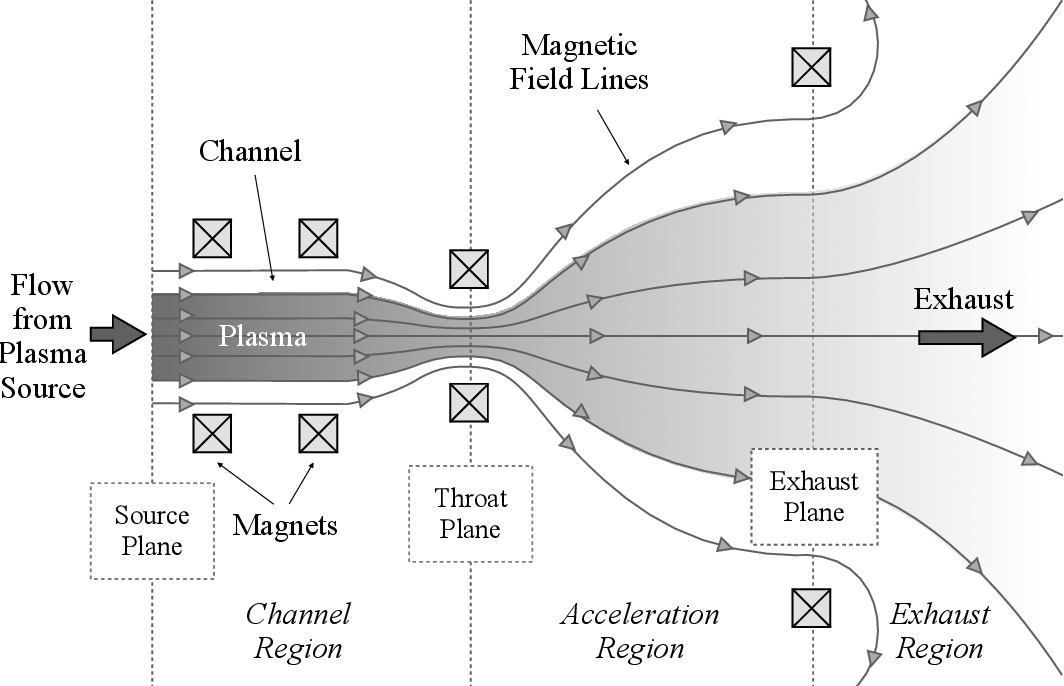
\includegraphics[width=0.7\linewidth]{../../thesis/img/introduction/magnetic-nozzle}
  \caption{A simplified model of the magnetic nozzle}
  \label{fig:magnetic-nozzle}
\end{figure}

\subsection{Magnetic Field in Magnetic Nozzle}
In 1D problem, the magnetic field can be modeled as
\[ B(z) = B_0 \left[1 + R\exp(-\left(\frac{x}{\delta}\right)^2)\right] \]
where $1+R$ is the magnetic mirror ratio, and $\delta$ determines the spread of the magnetic field. It is shown in Fig.(\ref{fig:magnetic-field}).
\begin{figure}[H]
	\centering
	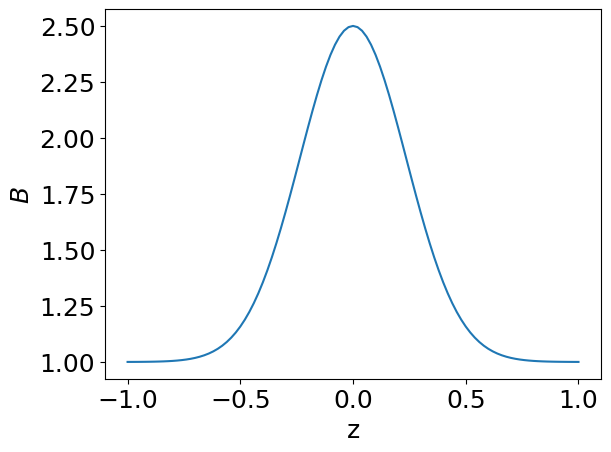
\includegraphics[width=0.7\linewidth]{../../thesis/img/introduction/magnetic-field}
	\caption{This is the magnetic field in nozzle with mirror ratio $1+R=B_{max}/B_{min}=2.5$, and the spread of magnetic field, $\delta=0.1/0.3=0.\bar{3}$. }
	\label{fig:magnetic-field}
\end{figure}

\subsection{Velocity Profile at Equilibrium}
Let $n_0$ and $v_0$ be the density and velocity at equilibrium (stationary solution), we know that $\pdv*{n_0}{t}=0$ and $\pdv*{v_0}{t}=0$, therefore $n_0$ and $v_0$ satisfy the so-called equilibrium condition,
\begin{align*}
	&\pdv{z}(\frac{n_0v_0}{B}) = 0 \\
	&v_0\pdv{v_0}{z} = -c_s^2\frac{1}{n_0}\pdv{n_0}{z} 
\end{align*}

Let $M(z) = v_0(z)/c_s$ be the mach number (nondimensionalized velocity). The equations of motion become
\begin{align*}
	&B\pdv{z}(\frac{n_0M}{B}) = 0\\
	&M\pdv{M}{z} = -\frac{1}{n_0}\pdv{n_0}{z}
\end{align*}
Substitute $\frac{1}{n_0}\pdv*{n_0}{z}$ using first equation, the conservation of momentum becomes
\[ (M^2-1)\pdv{M}{z} = -\frac{M}{B}\pdv{B}{z} \]

Notice that there is a singularity at $M=1$, the sonic speed.

This is a separable equation, integrate it and use the conditions at midpoint $B(0)=B_m, M(0)=M_m$ we get
\[ M^2e^{-M^2} = \frac{B^2}{B_m^2}M_m^2e^{-M_m^2} \]
We can now express $M$ using the Lambert W function,
\[ M(z) = \left[ -W_k\left(-\frac{B(z)^2}{B_m^2}M_m^2e^{-M_m^2}\right) \right]^{1/2} \]
where the subscript $k$ of $W$ stands for branch of Lambert W function. When $k=0$, it is the subsonic branch; When $k=-1$, it is the supersonic branch. Below shows a few cases of the solution.
\begin{itemize}
	\item $M_m < 1, k=0$, subsonic velocity profile.
	\item $M_m = 1$, $k=0$ for $x<0$ and $k=-1$ for $x>0$, accelerating profile
	\item $M_m = 1$, $k=-1$ for $x<0$ and $k=0$ for $x>0$, decelerating profile
	\item $M_m > 1, k=-1$, supersonic velocity profile
\end{itemize}
 Fig.(\ref{fig:velocity_profiles}) shows some cases of the solution.
\begin{figure}[H]
	\centering
	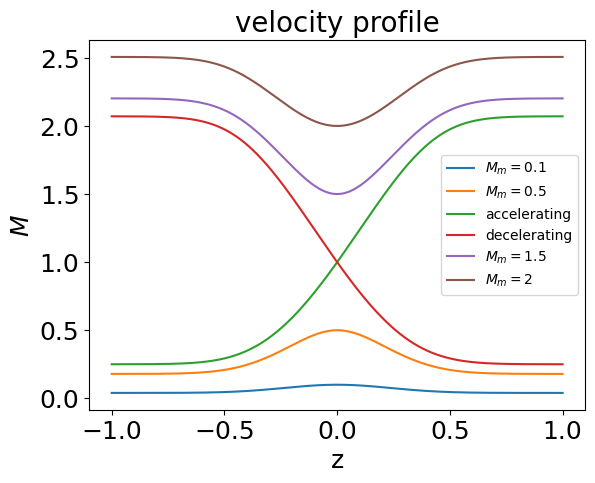
\includegraphics[width=0.7\linewidth]{../../thesis/img/introduction/velocity-profiles}
	\caption{The velocity profile in the magnetic nozzle is completely determined by $M_m$, the velocity at the midpoint, $z=0$. For the transonic velocity profiles, $M_m$ alone is not enough to determine the profile, we need to specify the branch of Lambert W function to determine whether it is accelerating or decelerating.}
	\label{fig:velocity_profiles}
\end{figure}

\subsection{Flow in Similar Configuration: Bondi-Parker Flow}
Bondi derived a steady-state solution for accretion flow which is governed by Bernoulli's equation in sperical symmetry around a point mass in 1952. Then Parker solved a similar problem but with outward wind in 1958. \cite{aikawa_stability_1979,bondi_spherically_1952,keto_stability_2020} The equilibrium velocity profiles in such configuration are shown in Fig.\ref{fig:BP-flow-velocity}.

\begin{figure}[htbp]
    \centering
    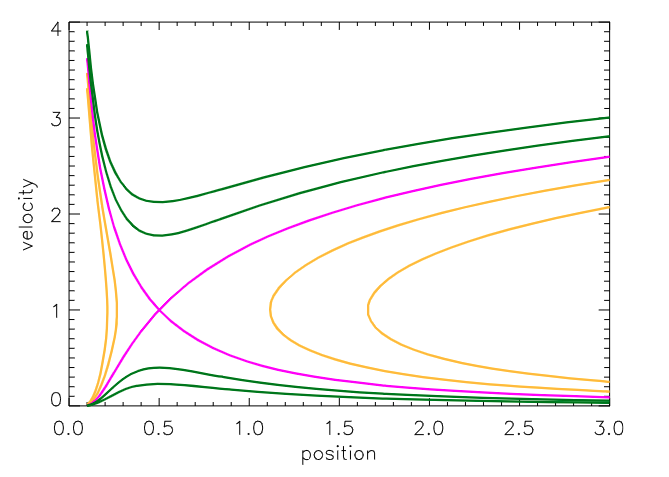
\includegraphics[width=0.7\textwidth]{../../thesis/img/introduction/steady-state-BP-flow}
    \caption{Representative trajectories of the steady-state BP flow in non-dimensional units. \cite{keto_stability_2020} The upward pink line represents a outward wind, it accelerates from subsonic to supersonic. The downward pink line represents an accretion flow, it accelerates towards the mass point. The green lines below the pink lines represent subsonic flows, and the green lines above represent supersonic flows. Orange lines are physically impossible scenarios.}
    \label{fig:BP-flow-velocity}
\end{figure}

Solar wind is an example of Bondi-Parker flow. The solar wind is a stream of charged particles, primarily electrons and protons, flowing outward from the Sun. 

\section{Instability of Plasma Flow}
In this section, plasma instability will be introduced and from that we will discuss the importance of this research.

The instability of plasma flow refers to the tendency of a plasma system to deviate from a stable, equilibrium state and exhibit perturbations or fluctuations in its behavior. These instabilities can arise from various factors, such as the interaction of particles with electromagnetic fields, collective effects, or the presence of gradients in plasma parameters.

\begin{figure}[htbp]
	\centering
	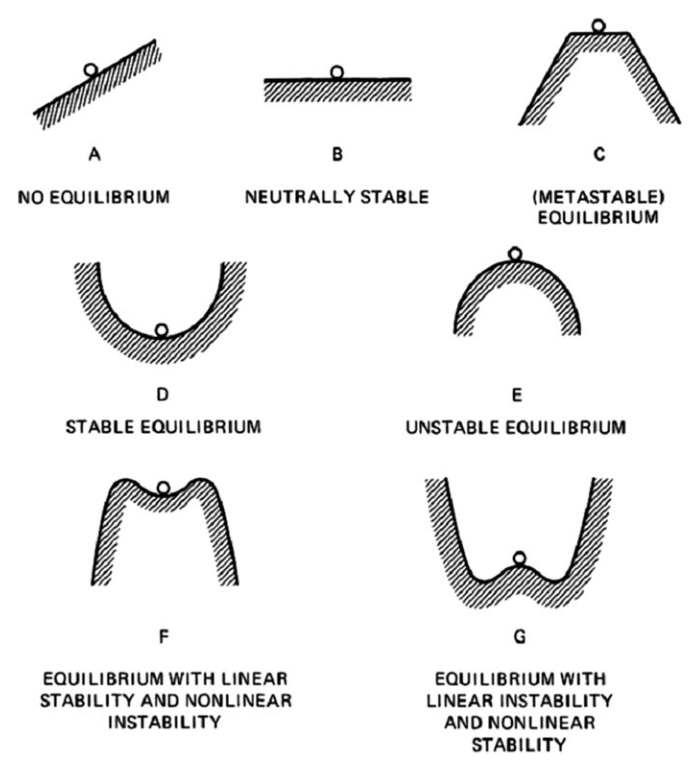
\includegraphics[width=0.7\linewidth]{../../thesis/img/introduction/stability-visualization}
	\caption{Mechanical analogy of various types of equilibrium. \cite{chen_introduction_2016}}
	\label{fig:stability-visualization}
\end{figure}

Plasma flow in magnetic mirror configurations have been studied extensively in plasma physics due to its frequent precense in many areas such as the accretion flow \cite{jockers_stability_1968,aikawa_stability_1979}, and magnetic nozzle\cite{smolyakov_quasineutral_2021}. However, the stability of these configurations remains a debatable subject.

\section{Goal of this Thesis}
The goal of this thesis is to study the instabilities of the magnetic mirror configuration given certain boundary conditions and equilibrium velocity profiles.

To achieve the goal, first we need to study the spectral method for solving the instability problem. To use spectral method, it is necessary to understand different discretizations of the operators, such as finite difference, finite element and spectral element method.

Once the spectral method is introduced, we can use it to study the instability of plasma flow in magnetic nozzle as an eigenvalue problem. We can obtain results by using different discretization techniques. By comparing the results from different approach, we can increase the credibility of the true solution.

However, spectral method is not suitable when the equilibrium velocity profile is transonic due to the precense of singularity at the sonic point. We need to solve the singular perturbation problem around the singularity analytically. Then starting from the singular point, we can use shooting method to find eigenvalues.

\section{Outline of the thesis}
The thesis will be divided into several chapters. In chapter 2, spectral method will be introduced. Chapter 3 will focus on the physics of flow in magnetic mirror configuration and derive the governing equations for charged particles, the linearized equations of motions. Following this, we will analyze the problem analytically in chapter 4. Moving to chapter 5, numerical experiments will be conducted. The conclusion will be made in chapter 6.
